% Fig. 1 block diagram. The paper includes the PDF built from this file with pdflatex.
\documentclass[10pt]{standalone}
\usepackage[T1]{fontenc}
\renewcommand{\rmdefault}{ptm}
\usepackage{amsmath,amssymb}
\usepackage{tikz}
\usetikzlibrary{arrows.meta}

\definecolor{ink}{HTML}{1A1A1A}
\definecolor{radarblue}{HTML}{1F4E9C}
\definecolor{radarred}{HTML}{B3261E}

\tikzset{
  block/.style={draw=ink, fill=white, line width=.5pt, rounded corners=.6mm, align=center, font=\footnotesize, inner sep=0pt},
  policy/.style={block, draw=radarblue, fill=radarblue!13},
  offline/.style={block, draw=radarred, fill=white},
  region/.style={line width=.5pt, rounded corners=1mm},
  flow/.style={-{Stealth[length=1.9mm,width=1.5mm]}, line width=.6pt, draw=ink},
  control/.style={flow, draw=radarblue},
  training/.style={flow, draw=radarred, dash pattern=on 1.5mm off .9mm},
  link/.style={-{Stealth[length=3mm,width=2.6mm]}, line width=1.5pt, draw=ink},
  tag/.style={font=\footnotesize, inner sep=.4mm},
  title/.style={font=\footnotesize\bfseries, anchor=west, fill=white, inner xsep=1mm, inner ysep=.2mm, rounded corners=.5mm},
}

% An IQ cube at (#1,#2), tinted with #3.
\newcommand{\iqcube}[3]{%
  \begin{scope}[shift={(#1,#2)}, scale=.8, line width=.45pt, draw=ink, line join=round]
    \filldraw[fill=#3!30] (-3.3,3.1) -- (-1.5,4.2) -- (4.3,4.2) -- (2.5,3.1) -- cycle;
    \filldraw[fill=#3!50] (2.5,3.1) -- (4.3,4.2) -- (4.3,-1.9) -- (2.5,-3) -- cycle;
    \filldraw[fill=#3!12] (-3.3,-3) rectangle (2.5,3.1);
    \draw[line width=.3pt] (-1.37,-3) -- (-1.37,3.1) (.57,-3) -- (.57,3.1) (-3.3,-.97) -- (2.5,-.97) (-3.3,1.07) -- (2.5,1.07);
  \end{scope}%
}

\begin{document}
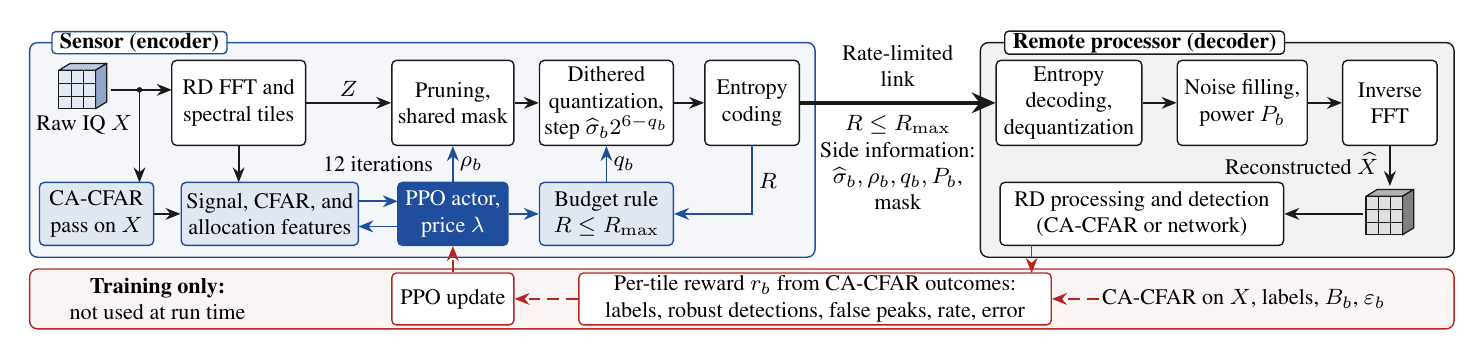
\begin{tikzpicture}[x=1mm, y=1mm]
\path[use as bounding box] (0,0) rectangle (181.4,38.5);

% Regions
\filldraw[region, draw=radarblue, fill=radarblue!5] (.25,9.35) rectangle (100,36.6);
\filldraw[region, draw=ink, fill=black!5] (121,9.35) rectangle (181.15,36.6);
\filldraw[region, draw=radarred, fill=radarred!5] (.25,.25) rectangle (181.15,7.85);
\node[title, draw=radarblue, line width=.5pt] at (3,36.6) {Sensor (encoder)};
\node[title, draw=ink, line width=.5pt] at (124,36.6) {Remote processor (decoder)};
\node[font=\footnotesize, align=center] at (16.5,4.05) {\textbf{Training only:}\\not used at run time};

% Signal path
\iqcube{6.6}{30.6}{radarblue}
\node[tag] at (7.2,26.2) {Raw IQ $X$};
\node[block, minimum width=17mm, minimum height=10.8mm] (fft) at (26.8,28.95) {RD FFT and\\spectral tiles};
\node[block, minimum width=15.5mm, minimum height=10.8mm] (prune) at (54,28.95) {Pruning,\\shared mask};
\node[block, minimum width=17mm, minimum height=10.8mm] (quant) at (73.5,28.95) {Dithered\\quantization,\\step $\widehat\sigma_b 2^{6-q_b}$};
\node[block, minimum width=12mm, minimum height=10.8mm] (code) at (92,28.95) {Entropy\\coding};
\node[block, minimum width=18.5mm, minimum height=10.8mm] (decode) at (132.25,28.95) {Entropy\\decoding,\\dequantization};
\node[block, minimum width=16.5mm, minimum height=10.8mm] (fill) at (154.25,28.95) {Noise filling,\\power $P_b$};
\node[block, minimum width=12mm, minimum height=10.8mm] (ifft) at (173,28.95) {Inverse\\FFT};
\draw[flow] (10.6,30.6) -- (18.3,30.6);
\draw[flow] (fft) -- node[tag, above, yshift=.3mm] {$Z$} (prune);
\draw[flow] (prune) -- (quant);
\draw[flow] (quant) -- (code);
\draw[link] (code) -- (decode);
\node[tag, align=center] at (110.5,33.6) {Rate-limited\\link};
\node[tag, align=center, anchor=north] at (110.5,27.8) {$R\le R_{\max}$\\Side information:\\$\widehat\sigma_b,\rho_b,q_b,P_b$,\\mask};
\draw[flow] (decode) -- (fill);
\draw[flow] (fill) -- (ifft);

% Output and detection
\iqcube{172.6}{14.6}{black}
\draw[flow] (173,23.55) -- (173,18.4);
\node[tag, anchor=east] at (172,21.2) {Reconstructed $\widehat X$};
\node[block, minimum width=36mm, minimum height=8mm] (detect) at (141.5,14.85) {RD processing and detection\\(CA-CFAR or network)};
\draw[flow] (169.6,14.85) -- (detect);

% Policy
\fill[ink] (14.2,30.6) circle (.35);
\draw[flow] (14.2,30.6) -- (14.2,18.85);
\node[policy, minimum width=14.5mm, minimum height=8mm] (cfar) at (8.75,14.85) {CA-CFAR\\pass on $X$};
\node[policy, minimum width=22.5mm, minimum height=8mm] (features) at (30.75,14.85) {Signal, CFAR, and\\allocation features};
\node[policy, minimum width=14mm, minimum height=8mm, text=white, fill=radarblue] (actor) at (54,14.85) {PPO actor,\\price $\lambda$};
\node[policy, minimum width=17mm, minimum height=8mm] (budget) at (73.5,14.85) {Budget rule\\$R\le R_{\max}$};
\draw[flow] (26.8,23.55) -- (26.8,18.85);
\draw[flow] (cfar) -- (features);
\draw[control] (42,16.45) -- (47,16.45);
\draw[control] (47,13.25) -- (42,13.25);
\node[tag] at (44.5,21.2) {12 iterations};
\draw[control] (actor) -- (budget);
\draw[control] (actor) -- node[tag, right, xshift=.4mm] {$\rho_b$} (prune);
\draw[control] (budget) -- node[tag, right, xshift=.4mm] {$q_b$} (quant);
\draw[control] (92,23.55) -- (92,14.85) -- (budget);
\node[tag, right, xshift=.4mm] at (92,19) {$R$};

% Training
\node[offline, minimum width=15.5mm, minimum height=6.6mm] (update) at (54,4.05) {PPO update};
\node[offline, minimum width=60mm, minimum height=6.6mm] (reward) at (100,4.05) {Per-tile reward $r_b$ from CA-CFAR outcomes:\\labels, robust detections, false peaks, rate, error};
\node[tag, anchor=west] (reference) at (136,4.05) {CA-CFAR on $X$, labels, $B_b$, $\varepsilon_b$};
\draw[training] (127.5,10.85) -- (127.5,7.35);
\draw[training] (reference) -- (reward);
\draw[training] (reward) -- (update);
\draw[training] (update) -- (actor);
\end{tikzpicture}
\end{document}
